%------------------------------------------%
% Cannabis Data Science #133
% Copyright (c) 2022 Cannlytics
% Date: 11/1/2023
%------------------------------------------%
\documentclass[xcolor={dvipsnames}]{beamer}
\hypersetup{pdfpagemode = FullScreen}
\mode<presentation>{
  \usetheme{Boadilla}
  \usecolortheme{orchid}
  \usefonttheme{default}
  \setbeamertemplate{navigation symbols}{}
  \setbeamertemplate{caption}[numbered]
}
\setbeamersize{
  text margin left = 0.5in,
  text margin right = 0.5in
}

%------------------------------------------%
% Title
%------------------------------------------%
\title[\textbf{Cannabis Data Science \#133}]{}
\author{Cannlytics}
\institute[]{\Large Cannabis Data Science \#133}
\date{November \nth{1}, 2023}

%------------------------------------------%
% Packages
%------------------------------------------%
\usepackage[english]{babel}
\usepackage[utf8x]{inputenc}
\usepackage{tikz} % For styling.
\usepackage{xparse}
\usepackage{amsmath}
\renewcommand*\footnoterule{} % No footnote line.
\usepackage{mathtools} % Annotating equations.
\usepackage{hhline} % Double bars.
\usepackage[super]{nth} % 1st, 2nd, 3rd, etc.
\usepackage{graphicx, caption, subcaption}
\usepackage{setspace}
\usepackage[charter]{mathdesign}
\usepackage{tikz}
\usetikzlibrary{tikzmark}
\usetikzlibrary{arrows.meta}

%------------------------------------------%
% Theme
%------------------------------------------%
\definecolor{LG}{RGB}{218, 247, 166}
\definecolor{DG}{RGB}{2, 48, 32}
\setbeamercolor*{palette primary}{bg=LG, fg=DG}
\setbeamercolor*{palette secondary}{bg=LG, fg=DG}
\setbeamercolor*{palette tertiary}{bg=LG, fg=DG}

%------------------------------------------%
% Commands
%------------------------------------------%

% Top space.
\newcommand\T{\rule{0pt}{2.5ex}}

% Bottom space.
\newcommand\B{\rule[-1.25ex]{0pt}{0pt}}

% Blocks.
\newenvironment<>{Block}[2][.9\textwidth]
  {\setlength{\textwidth}{#1}
  \begin{actionenv}#3
    \def\insertblocktitle{#2}\par
    \usebeamertemplate{block begin}}
  {\par\usebeamertemplate{block end}
  \end{actionenv}}

% Balls.
\defbeamertemplate{enumerate item}{largeball}
{\begin{pgfpicture}{-1ex}{-0.65ex}{1.5ex}{1.5ex}
\usebeamercolor[fg]{item projected}
{\pgftransformscale{2.5}\pgftext{\Large\pgfuseshading{bigsphere}}}
{\pgftransformshift{\pgfpoint{0pt}{0.5pt}}
\pgftext{\usebeamerfont*{item projected}\small\insertenumlabel}}
\end{pgfpicture}}

% Fancy arrows.
\NewDocumentCommand\UpArrow{O{2.0ex} O{black}}{%
   \mathrel{\tikz[baseline] \draw [->, line width=0.5pt, #2] (0,0) -- ++(0,#1);}} % Fancy up-arrow.
\NewDocumentCommand\DownArrow{O{2.0ex} O{black}}{%
   \mathrel{\tikz[baseline] \draw [<-, line width=0.5pt, #2] (0,0) -- ++(0,#1);}} % Fancy down-arrow.

% Equations with numbers on the left.
\makeatletter
\newcommand{\LeftEqNo}{\let\veqno\@@leqno}
\makeatother

% Print out title.
\defbeamertemplate*{title page}{customized}[1][]
{
  \usebeamerfont{title}\inserttitle\par
  \bigskip
  \vspace{0.5\baselineskip}
  \usebeamerfont{institute}\insertinstitute\par
  \vspace{0.5\baselineskip}
  {\small\usebeamerfont{date}\insertdate\par}
  \usebeamercolor[fg]{titlegraphic}\inserttitlegraphic
}

%------------------------------------------%
%
% Presentation
%
%------------------------------------------%
\begin{document}

% Title page.
\begin{frame}{}

% Background
\tikz[remember picture, overlay]
\node[opacity=1.0, inner sep=0pt] at (current page.center){
  
\includegraphics[height=\paperheight, width=\paperwidth]{images/presentation-cover.pdf}
};

% Title
\vspace*{4\baselineskip}

\includegraphics[scale=0.375]{images/logo.pdf}
\vspace*{-2\baselineskip}
\titlepage
\end{frame}


%------------------------------------------%
% Icebreaker
%------------------------------------------%


\begin{frame}

\begin{center}
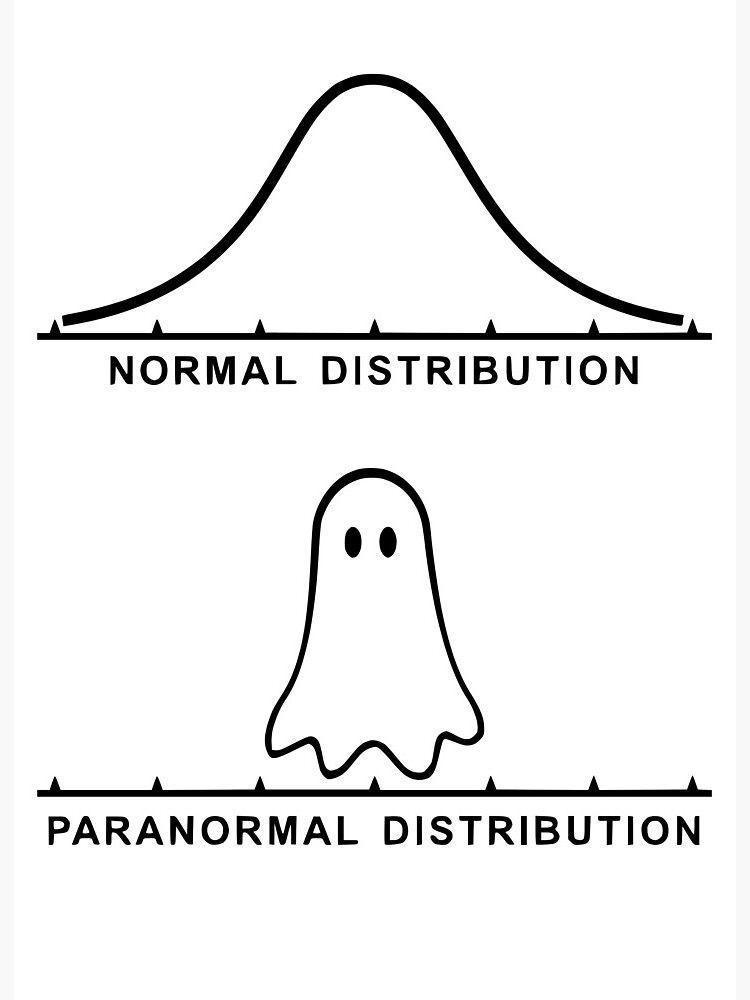
\includegraphics[width=0.7\linewidth]{images/paranormal-distribution.png}
\end{center}

\end{frame}


\begin{frame}

\begin{center}
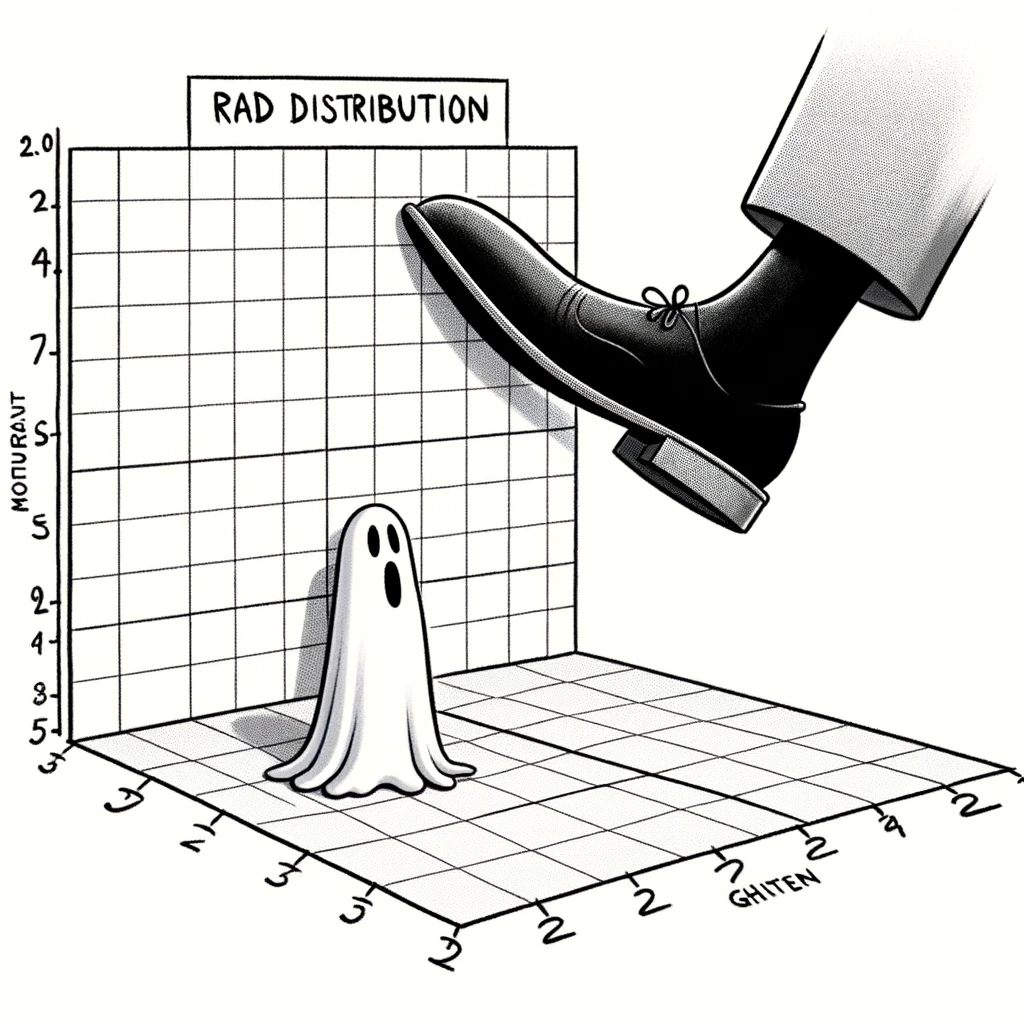
\includegraphics[width=0.88\linewidth]{images/rad-distribution.png}
\end{center}

\end{frame}


%------------------------------------------%
% Introduction
%------------------------------------------%

\begin{frame}{Cannabis Data Science Application}

\begin{center}
\begin{minipage}{3.85in}

% Thank you.

\begin{center}
\begin{minipage}{\linewidth}
\begin{Block}{Question of the Day}

\vspace{0.5\baselineskip}

\begin{itemize}

\item Is it possible to quantify the {\bfseries diversity} of cannabis products in a market?


\vspace{0.75\baselineskip}

\end{itemize}

\end{Block}
\end{minipage}
\end{center}

\vfill

\end{minipage}
\end{center}

\end{frame}

%------------------------------------------%
% Literature Review
%------------------------------------------%

%\begin{frame}
%\frametitle{Introduction}
%\begin{itemize}
%    \item {\bfseries Approach}:
%    \begin{enumerate}
%    \item Identify established diversity indices.
%    \item Calculate diversity metrics.
%    \item Test if diversity metrics change over time.
%    \end{enumerate}
%\end{itemize}
%\end{frame}

\begin{frame}
\frametitle{Diversity Measures}
\begin{itemize}
\item {\bfseries Abundance} - Quantity of each species.
\vspace{1em}
\item {\bfseries Evenness} - Commonness or rarity of species.
\vspace{1em}
\item {\bfseries Dominance} - The degree of species size.
\vspace{1em}
\item {\bfseries Richness} - A simple count of species.

\end{itemize}
\end{frame}


%    \item A quantitative measure reflecting the number of different types in a dataset.
%    \item Considers richness, divergence, and evenness.
%    \item Accounts for both categorical and qualitative diversity.

\begin{frame}
\frametitle{Hill Numbers}
%Explains how the diversity indices can be interpreted as the effective number of types (species, products) in a dataset.
The {\bfseries general equation of diversity} is:
\vspace{0.5em}
$$
{}^{q}D = \left(\sum_{i=1}^{R}p_{i}^{q}\right)^{1/(1-q)}
$$
Where:
\vspace{1em}
\begin{itemize}
\item \(R\) is richness,
\vspace{0.5em}
\item \(p_i\) is the proportional abundance of the \(i\)th type,
\vspace{0.5em}
\item \(q\) is the sensitivity of the diversity value to rare and abundant species.
\end{itemize}

\end{frame}


\begin{frame}
\frametitle{Diversity Metrics}

\begin{itemize}
\item {\bfseries Shannon Index} - Quantifies uncertainty in predicting the species of a randomly chosen observation.
\[ H' = -\sum_{i=1}^{R}p_{i}\ln(p_{i}) \]
\vspace{1em}
\item {\bfseries Simpson Index} - Measures the degree of concentration of species.
\[ \lambda = \sum_{i=1}^{R}p_{i}^{2} \]
\end{itemize}

\end{frame}

%------------------------------------------%
% Data
%------------------------------------------%



%------------------------------------------%
% Methods
%------------------------------------------%

\begin{frame}
\frametitle{Rank abundance curve}

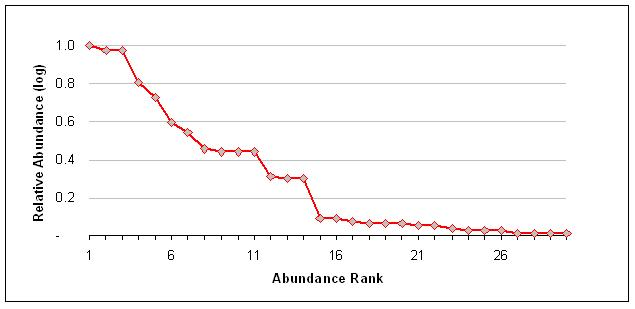
\includegraphics[width=\linewidth]{images/rank-abundance.jpg}

\begin{itemize}

\item {\bfseries Richness} can be viewed as the number of different species.

\item {\bfseries Evenness} is reflected in the slope. Steeper gradients indicates lower evenness. 

\end{itemize}

\end{frame}


%Rank abundance curve
% The rank abundance curve visually depicts both species richness and species evenness. Species richness can be viewed as the number of different species on the chart i.e., how many species were ranked. Species evenness is reflected in the slope of the line that fits the graph (assuming a linear, i.e. logarithmic series, relationship). A steep gradient indicates low evenness as the high-ranking species have much higher abundances than the low-ranking species. A shallow gradient indicates high evenness as the abundances of different species are similar.

%------------------------------------------%
% Takeaway
%------------------------------------------%
\section{Takeaway}

\begin{frame}{}

\vspace{0.5\baselineskip}

\begin{center}
\begin{minipage}{3.85in}

% Thank you.

\includegraphics[width=.25in]{images/prayer.png} {\Large \textbf{Thank you for coming.}}\\[-0.75\baselineskip]

\begin{center}
\begin{minipage}{\linewidth}
\begin{Block}{Insight of the Day}

\vspace{0.5\baselineskip}

\begin{itemize}

\item Ask and you shall receive.

\vspace{0.75\baselineskip}

\end{itemize}

\end{Block}
\end{minipage}
\end{center}

\vfill

\end{minipage}
\end{center}

\vspace{0.5\baselineskip}

{\large What is on your mind for next week?}\\

\end{frame}


%------------------------------------------%
% Fin.
%------------------------------------------%
\end{document}
